\chapter{La Gestion des Stocks}

\section{La page "Matières Premières"}
Cette page liste les matières premières par ordre alphabétique. Pour chaque 
matière première sont affichés son nom et sa quantité disponible.

\subsection{Affichage des matières premières}

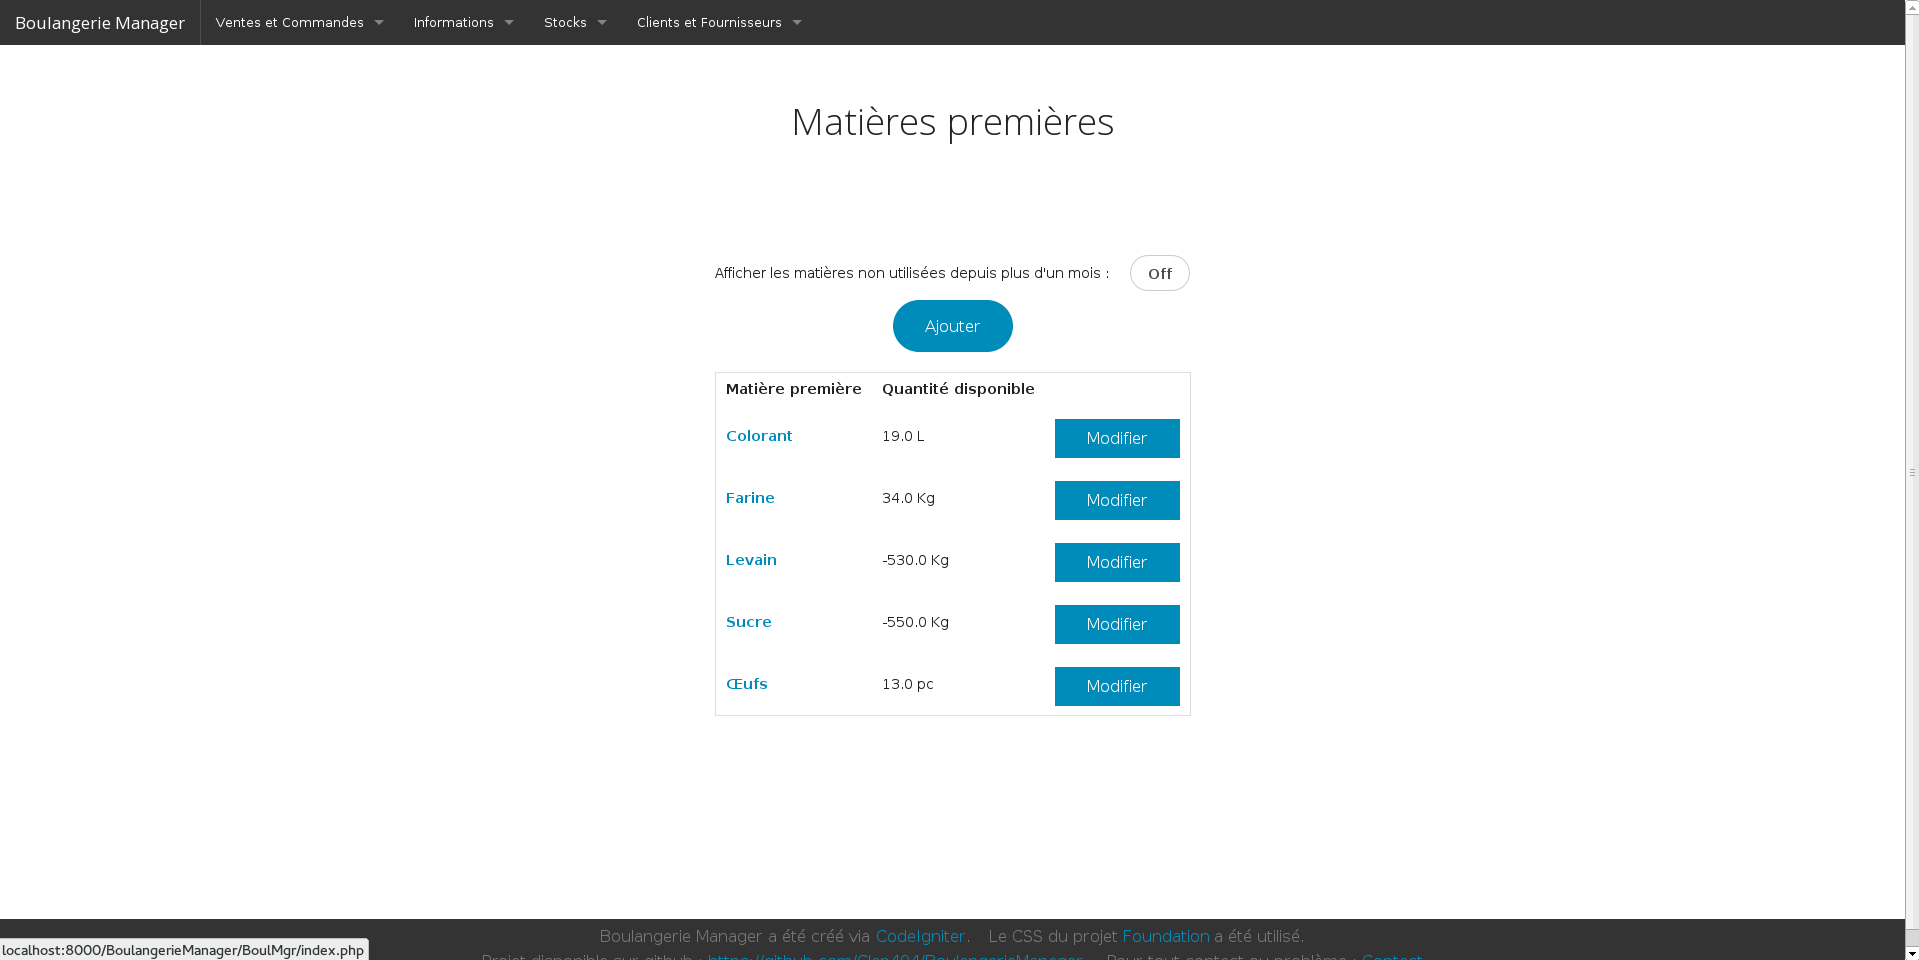
\includegraphics[scale=0.30]{matprem1.png}\\

Sur la page "Matières Premières" se site un bouton qui permet d'afficher ou non 
certaines matières premières. Quand ce bouton est désactivé (OFF), les matières 
premières non utilisées depuis plus d'un mois ne sont pas visibles. Si ce bouton
 est activé (ON), ces dernières sont visibles dans le tableau.


\subsection{Ajout d'une matière première}
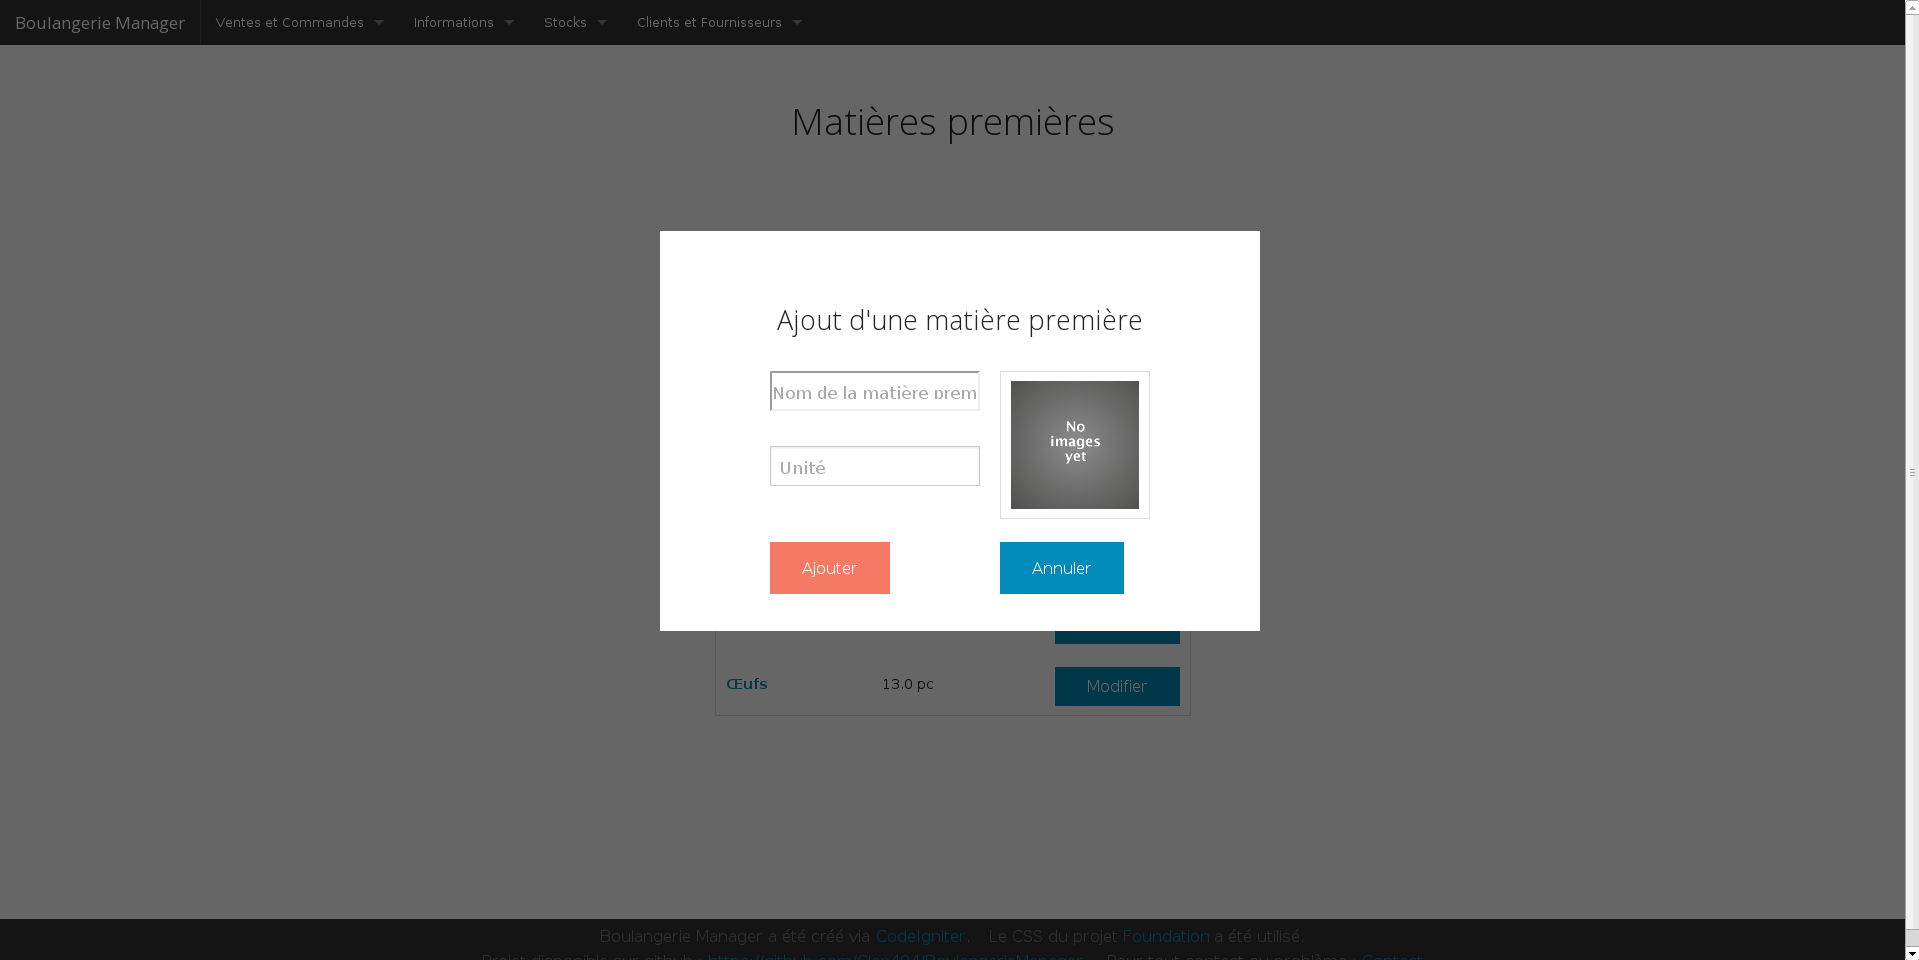
\includegraphics[scale=0.30]{matprem2.png}\\
Sur la page "Matières Premières", la liste des matières est précédée d'un bouton
 "Ajouter". 
Un clic sur ce bouton "Ajouter" fait apparaitre une fenêtre au premier plan. 

\paragraph{}
Sur cette fenêtre sont présents deux champs à remplir. Le premier est le nom de 
la matière première à ajouter, le deuxième représente l'unité dans laquelle la 
matière première est exprimée. Il est également possible d'associer à cette 
matière première une image la représentant. En cliquant sur le cadre dédié à 
l'image, il est possible de charger une image depuis son ordinateur. L'image est
un élément facultatif. Tant que les deux premiers champs ne sont pas remplis, 
le bouton "Ajouter" est bloqué et coloré en rouge. Pour ajouter une matière 
première, il suffit de remplir ces deux champs et de cliquer sur le bouton 
"Ajouter". Un clic sur le bouton "Annuler" ou en dehors de la fenêtre ferme 
le formulaire d'ajout d'une matière première.


\subsection{Modification du nom d'une matière première}
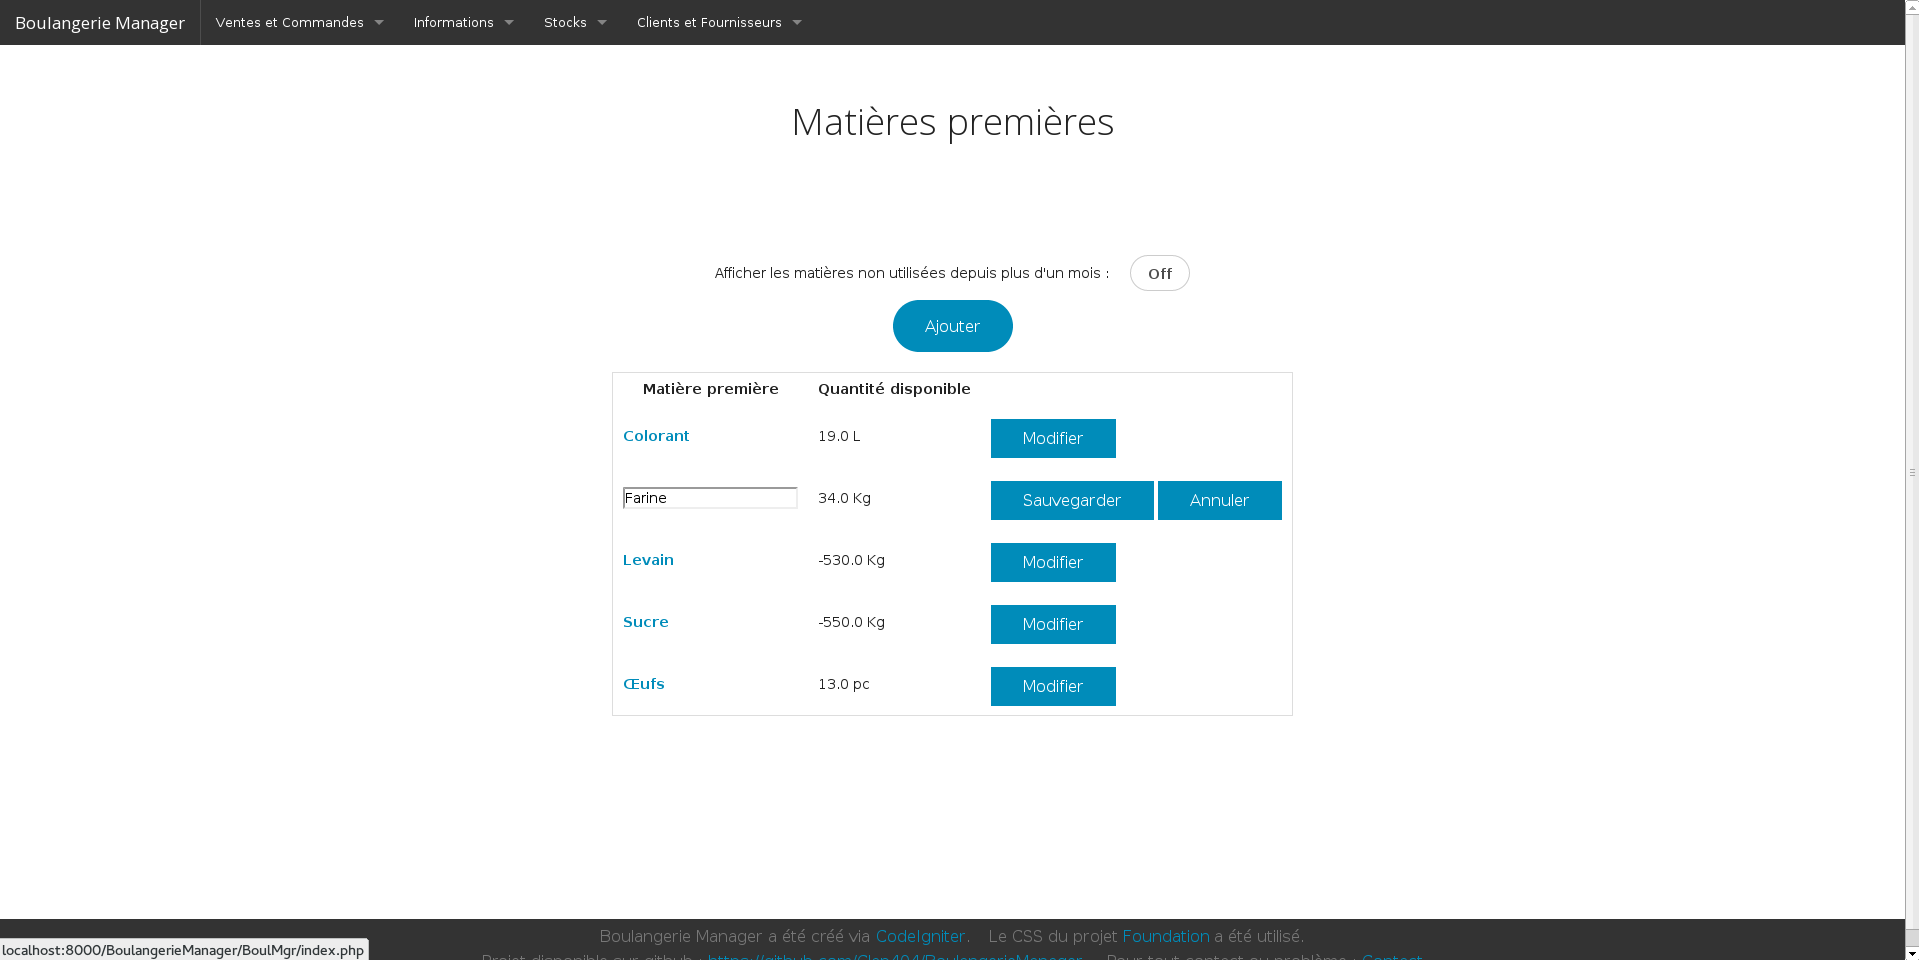
\includegraphics[scale=0.30]{matprem3.png}\\
Sur la page "Matières Premières" se trouve, pour chaque matière première, 
un bouton "Modifier". Un clic sur ce bouton permet de modifier une matière 
première.

\paragraph{}
Après avoir cliqué sur le bouton "Modifier" présent sur la page "Matières 
Premières", on voit apparaitre un champ dans lequel on peut renseigner un 
nouveau nom pour une matière première. Si le nom n'est pas renseigné ou est 
égal à celui déjà présent, une erreur s'affiche. Sinon, en cliquant sur le 
bouton "Sauvegarder", le nom de la matière première est modifié. Un clic sur 
le bouton "Annuler" ferme le formulaire de modification.


\subsection{Détails d'une matière première}
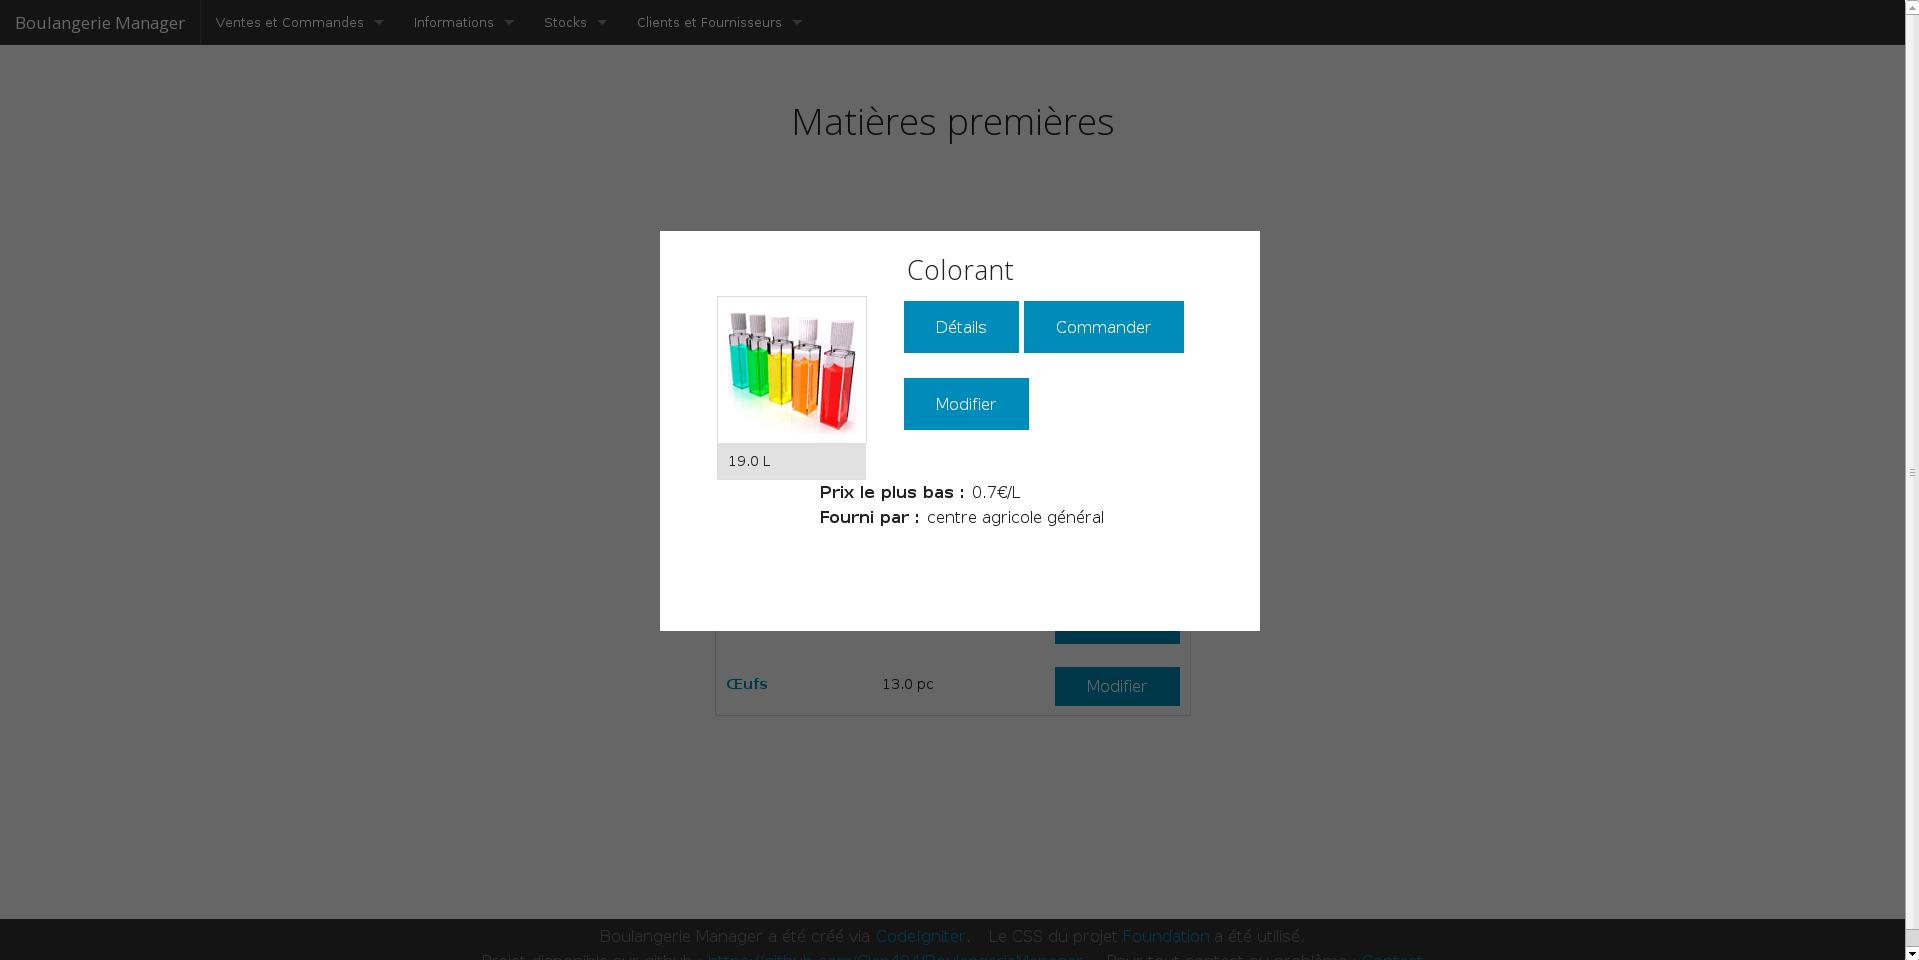
\includegraphics[scale=0.30]{matprem4.png}\\
Pour chaque matière première listée dans le tableau de la page "Matières 
Premières", il est possible d'accéder à des détails. Un clic sur le nom d'une 
matière première fait apparaitre une fenêtre au premier plan.

\paragraph{}
Sur cette fenêtre sont renseignés le nom de la matière première, l'image qui lui 
est associée, sa quantité disponible en stock, son prix le plus bas à l'achat, 
ainsi que le fournisseur qui a livré la dernière commande de ce produit.

\subsection{Modification plus détaillée d'une matière première}
Lorsque l'on se trouve sur la fenêtre qui détaille les matières premières
(section précédente), il est possible de modifier une matière première en 
cliquant sur le bouton "Modifier".

\paragraph{}
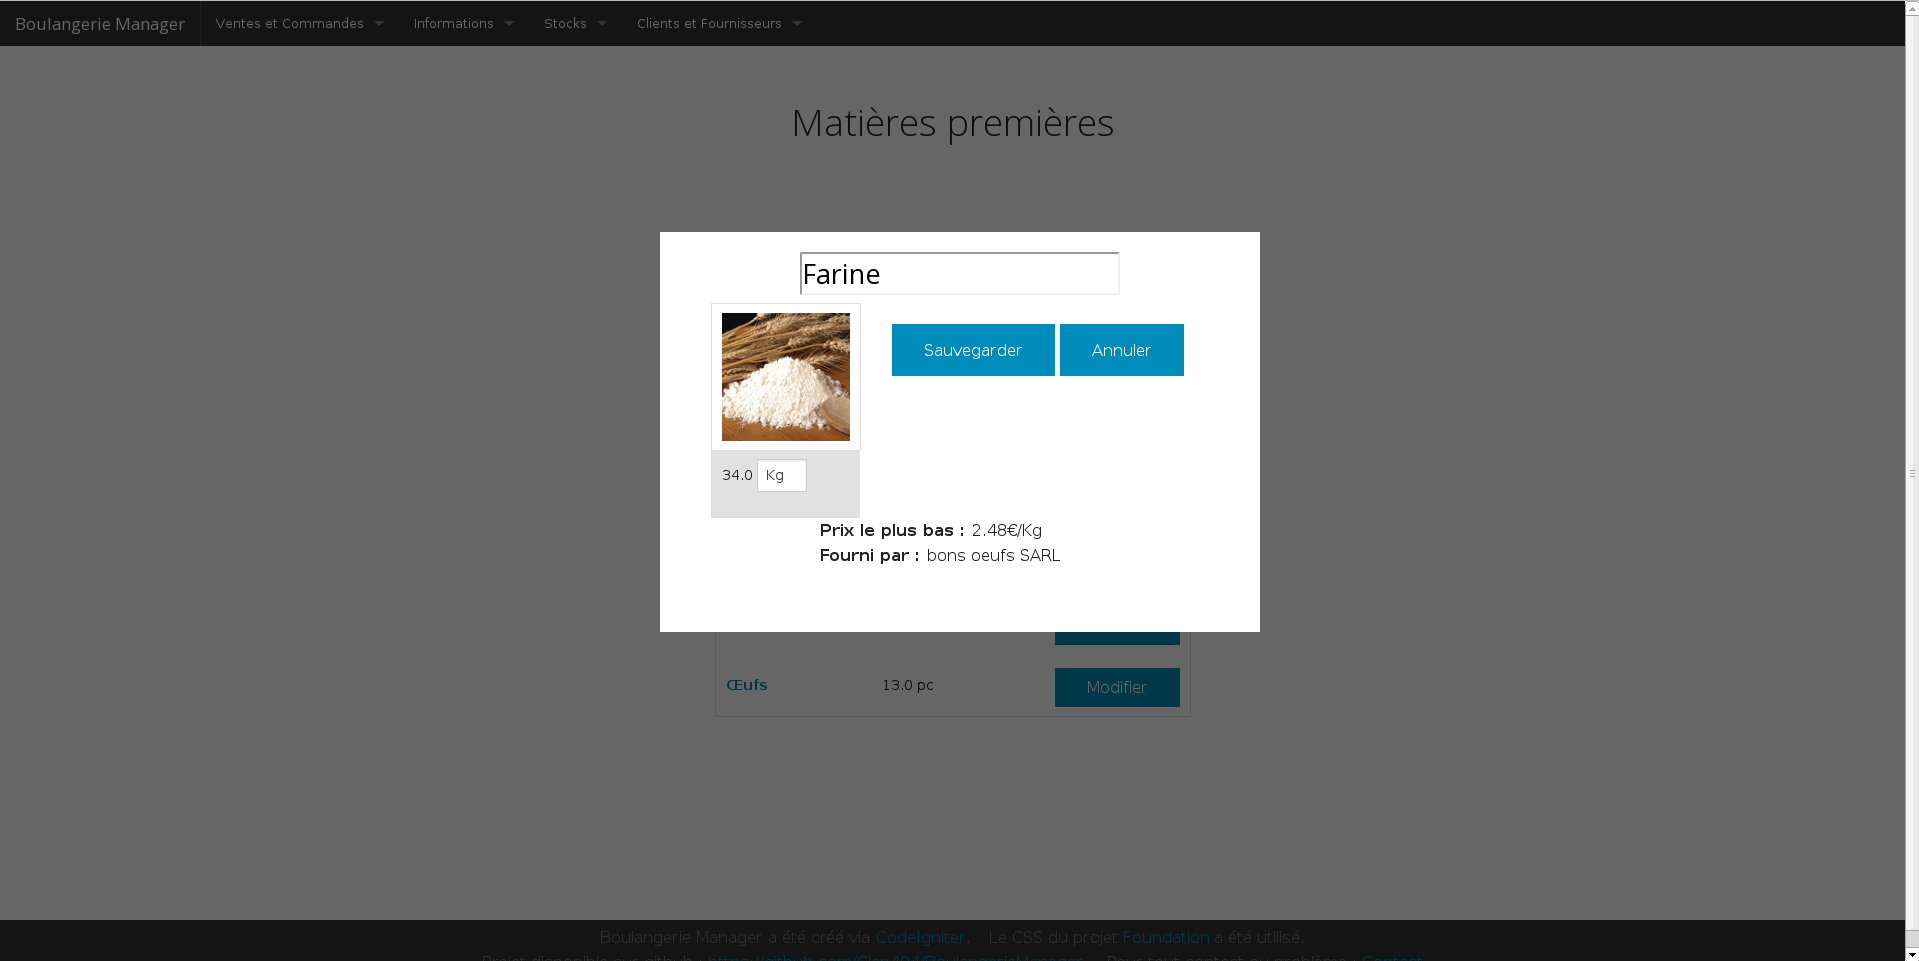
\includegraphics[scale=0.30]{matprem5.png}\\
Après avoir cliqué sur le bouton "Modifier", deux champs apparaissent. Le 
premier permet de modifier le nom de la matière première choisie. Le deuxième, 
situé en bas de l'image, permet de modifier l'unité dans laquelle la matière 
première est exprimée. Sur cette fenêtre est également possible de modifier 
l'image associée à la matière première en cliquant sur l'image déjà présente. 
Ce clic permettra de charger une image depuis son ordinateur. Pour sauver les 
modifications effectuées, il suffit de cliquer sur le bouton "Sauvegarder". Si 
tous les champs sont remplis, la fenêtre va se recharger avec les nouvelles 
informations. Sinon, une erreur apparaitra sur cette même fenêtre.

\subsection{Commande d'une matière première}
Sur la même fenêtre que précédemment se trouve également un bouton "Commander". 
Ce bouton permet de commander la matière première au fournisseur associé.

\paragraph{}
Après avoir cliqué sur le bouton "Commander", un champ apparait afin de 
permettre à l'utilisateur de renseigner la quantité qu'il veut commander. 
En fonction de la quantité renseignée, le prix que cette commande va couter 
s'affiche en dessous de la quantité demandée, afin de permettre à l'utilisateur 
d'avoir une idée du prix auquel cette commande va lui revenir. Lorsque la 
quantité est renseignée par l'utilisateur, le bouton "Sauvegarder" devient 
actif. Un clic sur ce bouton remet en stock la quantité de matière première 
commandée et inscrit la commande dans la partie "Commande" de l'application.

\subsection{Page détaillée d'une matière première}
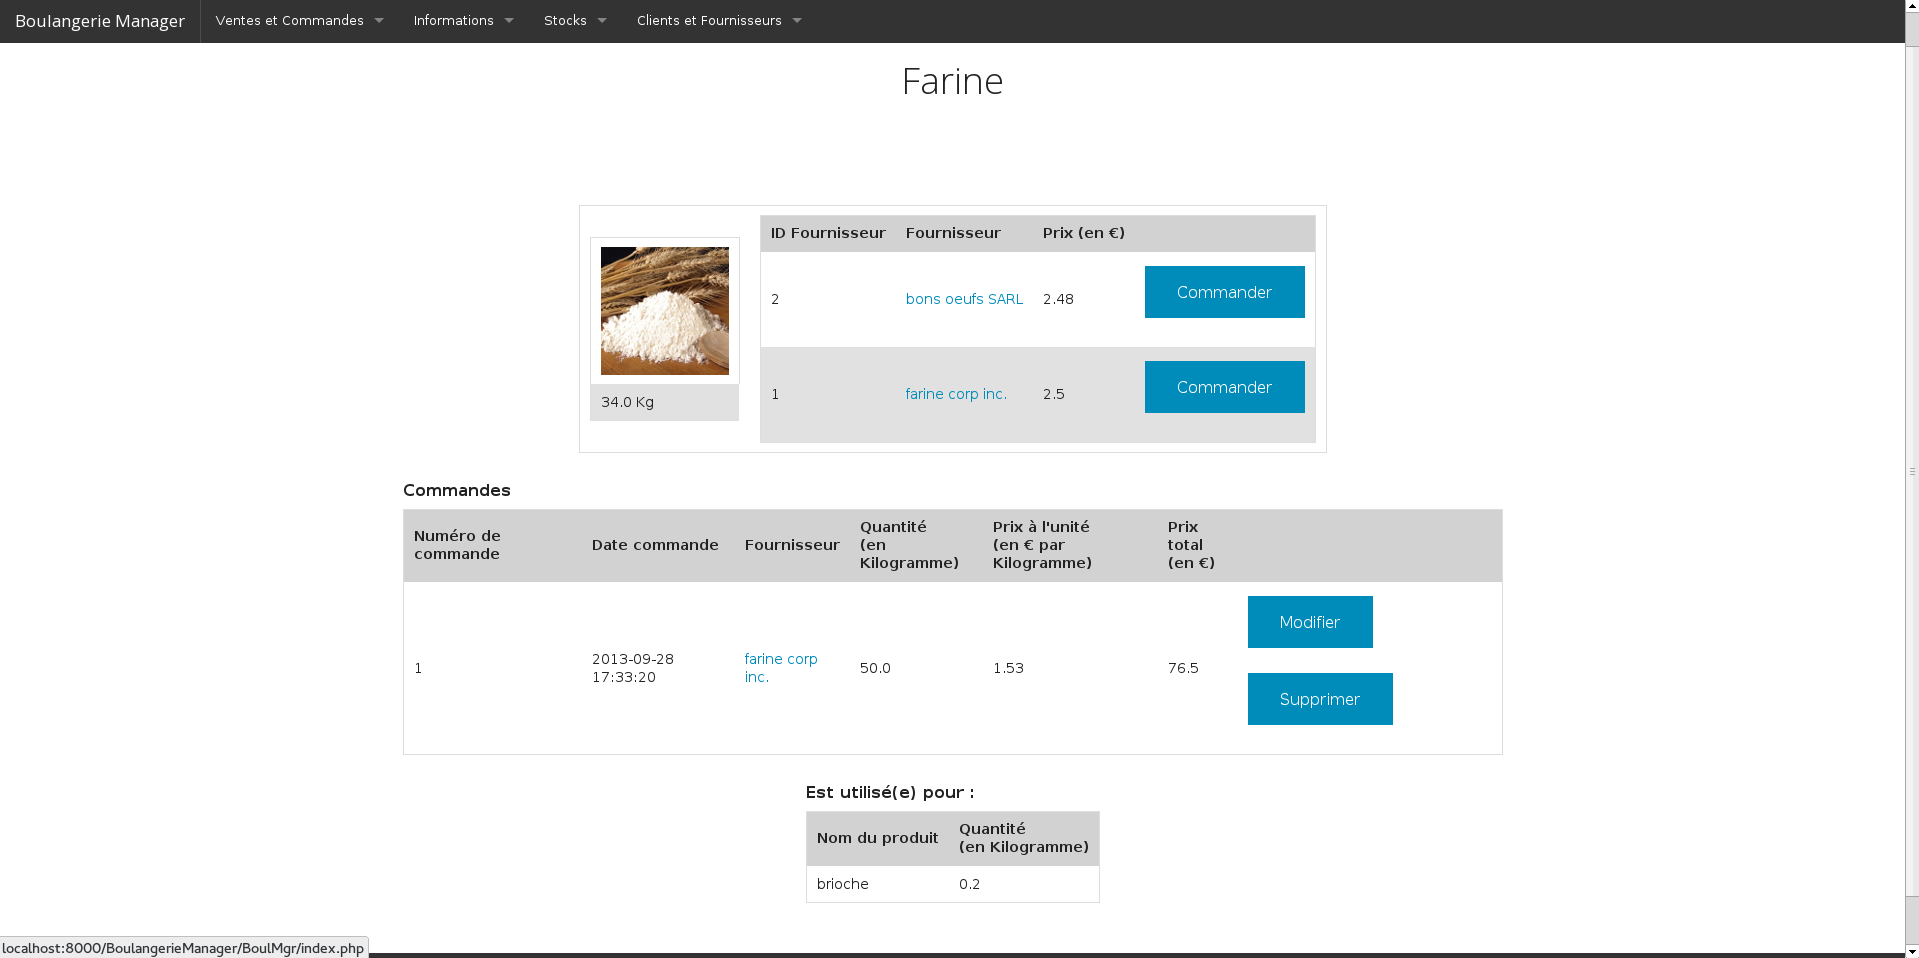
\includegraphics[scale=0.30]{matprem6.png}\\
A l'ouverture des détails d'une matière première, un bouton "Détails" apparait. 
Après avoir cliqué sur ce bouton, une page dédiée à une matière première 
s'ouvre. 

\paragraph{}
Sur cette page se retrouvent les éléments caractéristiques d'une matière 
première. Son image associée, son nom, ainsi que sa quantité disponible sont 
présents. A la suite de ces informations se situe un tableau présentant les 
différents fournisseurs pouvant fournir cette matière première, avec le prix 
associé à celle ci. Un bouton "Commander" est également présent qui agit de la 
même façon que précédemment.

\paragraph{}
Sous ce tableau se trouvent les commandes qui ont été passées aux différents 
fournisseurs qui traitent de cette matière première. Pour ces commandes sont 
renseignées :
\begin{enumerate}
  \item \textbf{Le numéro de la commande}
  \item \textbf{La date de la commande}
  \item \textbf{Le fournisseur associé} : Un clic sur le nom du fournisseur 
  associé permet d'ouvrir la page associée à celui-ci. Le contenu de cette page 
  est détaillé dans la section "Fournisseurs".
  \item \textbf{La quantité commandée}
  \item \textbf{Le prix unitaire de la matière première}
  \item \textbf{Le prix total en €}
  \item \textbf{Un bouton "Modifier"} : Un clic sur ce bouton fait apparaitre 
  une fenêtre au premier plan. Dans cette fenêtre se trouvent les éléments 
  caractéristiques de la commande à modifier. Son fournisseur, le prix unitaire 
  de la matière première commandée, la quantité commandée et le prix total.
  Seule la quantité commandée est modifiable dans cette fenêtre. Avec une 
  modification de la quantité, le prix total est également recalculé 
  directement dans cette même fenêtre. Il suffit ensuite de cliquer sur le 
  bouton "Valider" pour appliquer les modifications.

  \item \textbf{Un bouton "Supprimer"} : Ce bouton permet de supprimer une 
  commande. En cliquant sur ce bouton, une fenêtre de confirmation apparait, 
  demandant si l'utilisateur veut ou non confirmer la suppression.
\end{enumerate}

\paragraph{}
Sous le tableau des commandes se trouve un autre tableau. Celui-ci permet de 
voir dans quelle préparation la matière première en question est utilisée. Dans 
ce tableau est présent le nom du produit qui nécéssite cette matière première, 
ainsi que la quantité nécéssaire afin de le produire.



\section{La page "Produits"}
Cette page liste les produits. Pour chaque produits sont affichés son nom, sa 
quantité disponible ainsi que son temps de préparation.

\paragraph{}
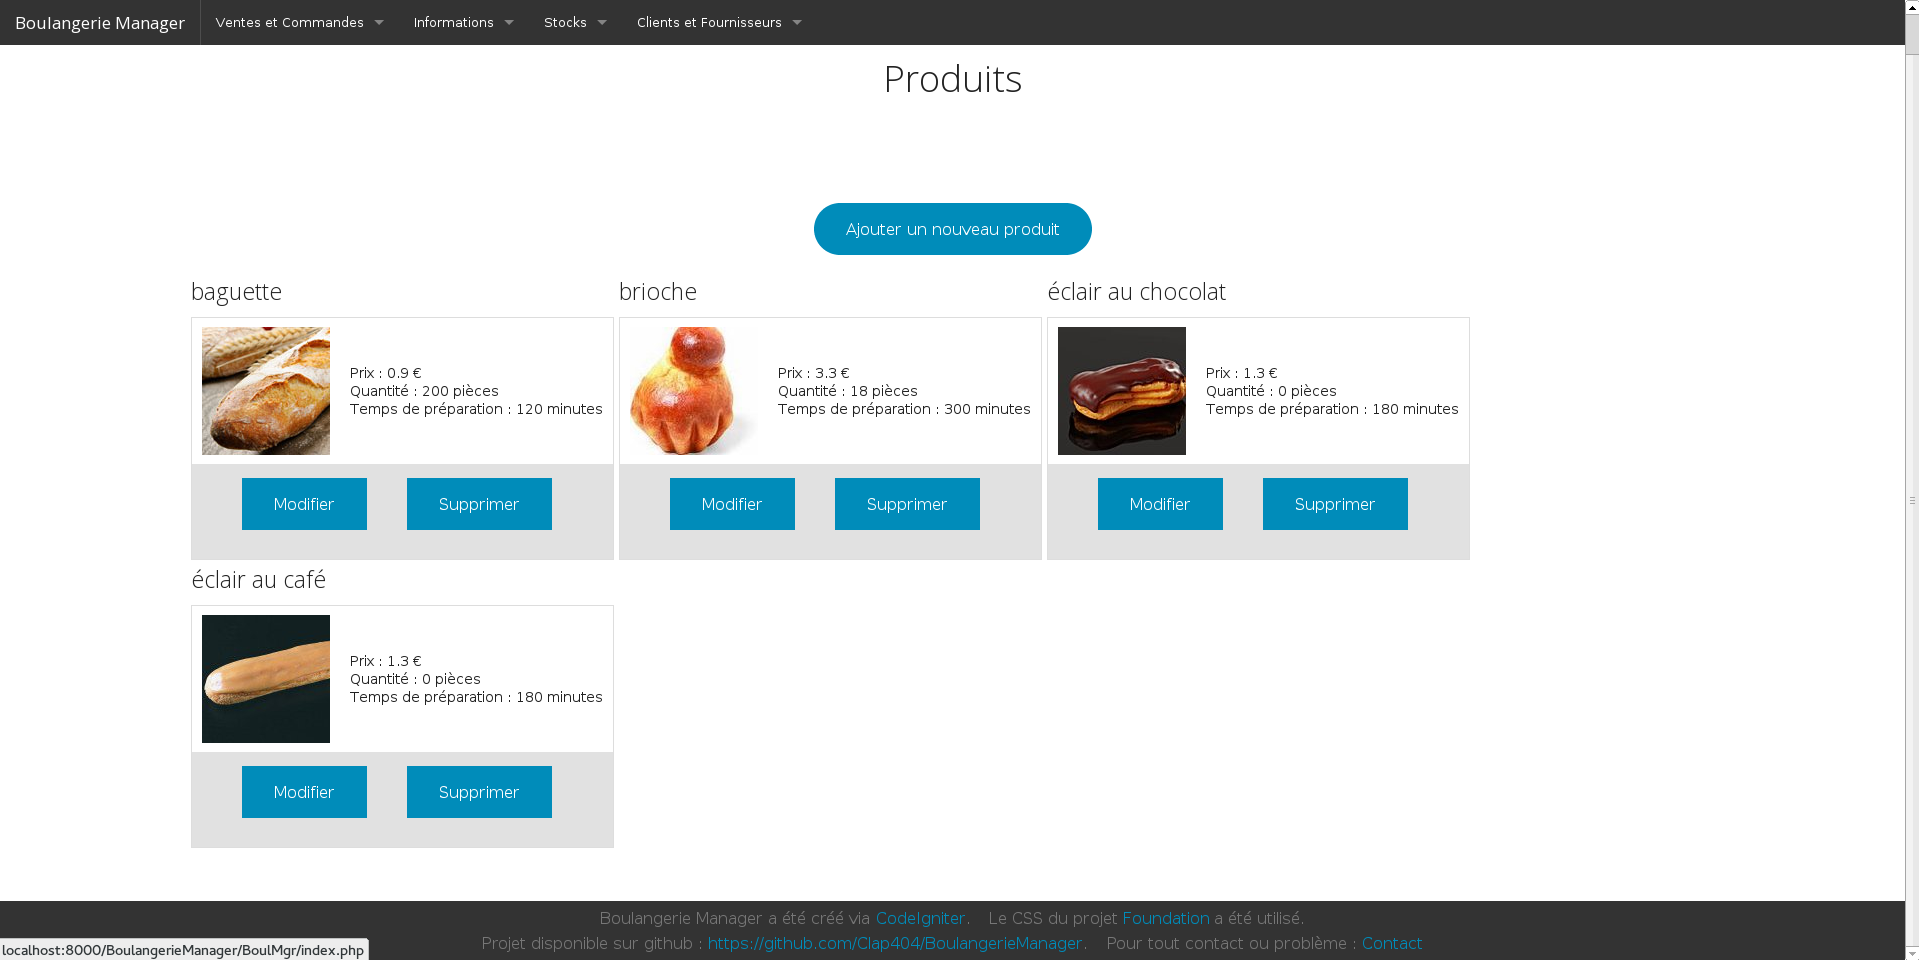
\includegraphics[scale=0.30]{produit1.png}\\
Chaque produit est affiché sous forme de "vignette". Au dessus de chaque 
vignette se trouve le nom du produit. Dans une vignette on retrouve le prix du 
produit à l'unité, la quantité disponible en stock, ainsi que le temps nécéssaire 
à sa préparation. Dans le bas de chaque vignette se trouvent deux boutons : 
"Modifier" et "Supprimer".

\subsection{Modification d'un produit}
En cliquant sur le bouton "Modifier" d'un produit, une page de modification 
s'ouvre. 

\paragraph{}
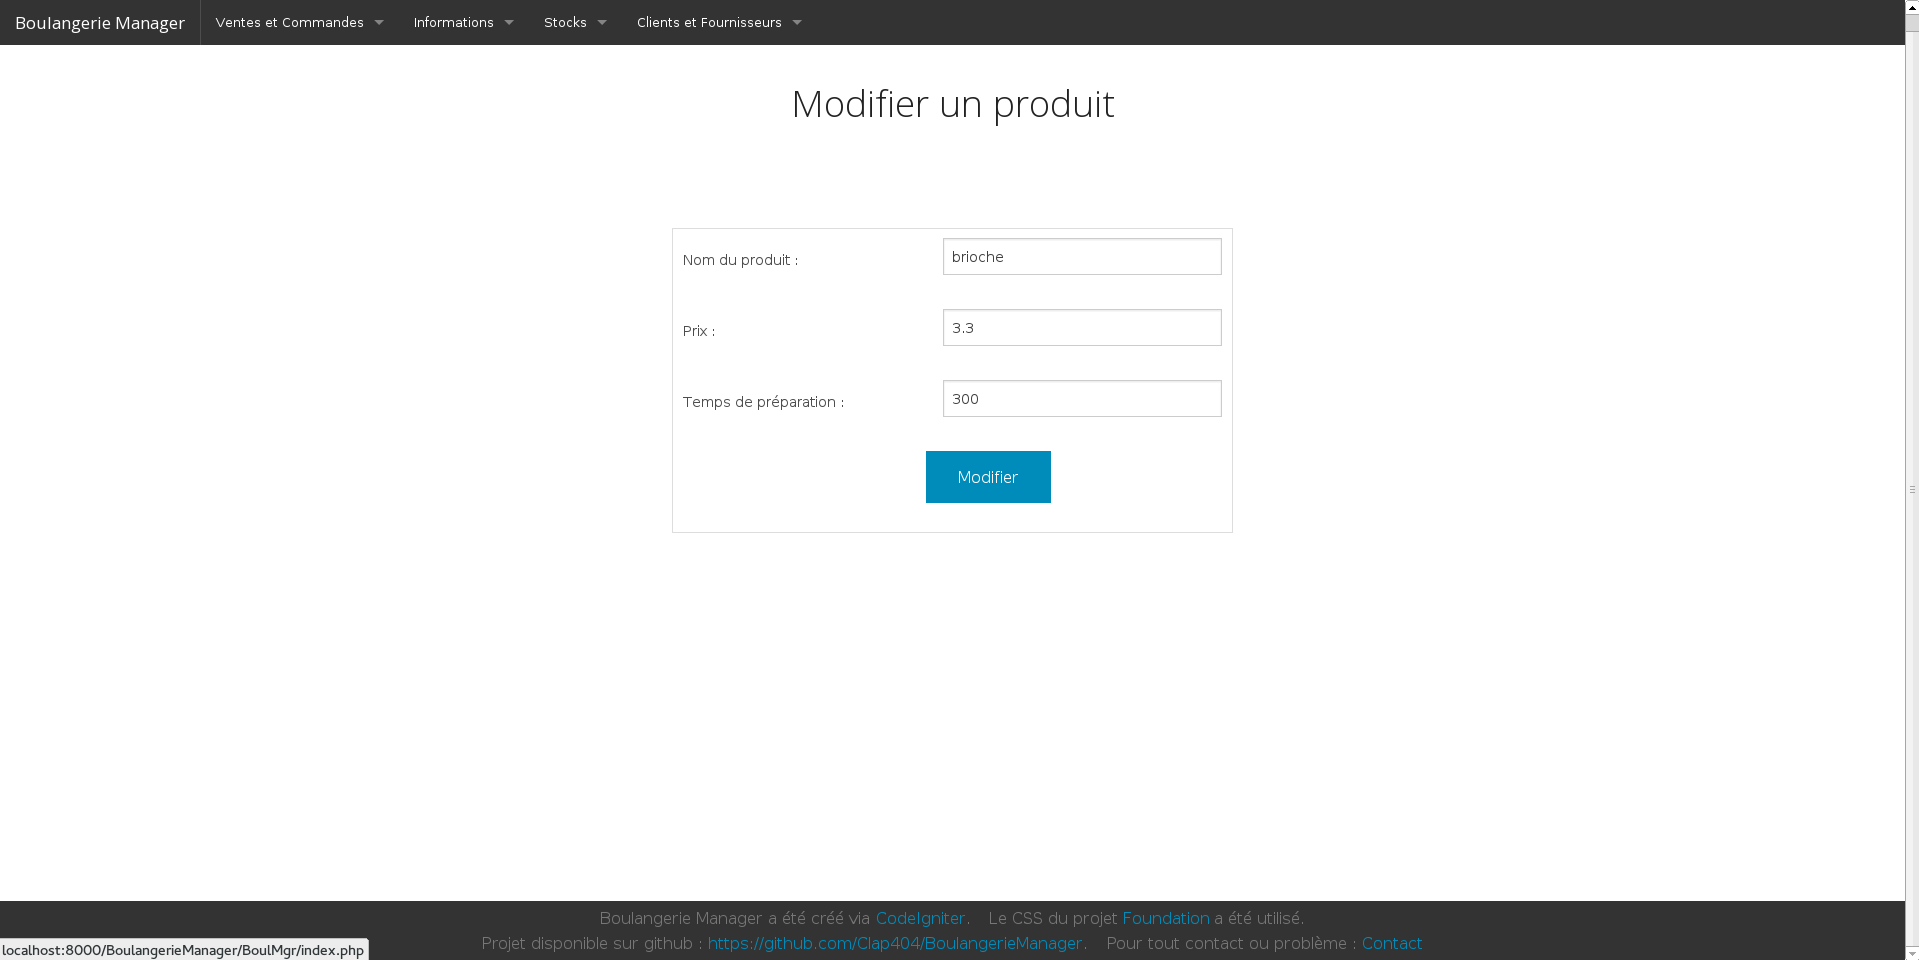
\includegraphics[scale=0.30]{produit2.png}\\
Sur cette page de modification se trouvent trois champs à remplir. 
Le premier correspond au nom du produit, le deuxième au prix unitaire du produit, 
et le troisième représente son temps de préparation. Il est possible de modifier 
au choix une, deux ou trois caractéristiques du produit. Si l'un des trois champs 
n'est pas rempli, lorsque l'on clique sur le bouton "Modifier", une erreur 
détaillant quel champ n'est pas renseigné apparaitra. Mais si les trois champs 
sont renseignés correctement, un simple clic sur le bouton "Modifier" permettra 
de modifier le produit.

\subsection{Suppression d'un produit}
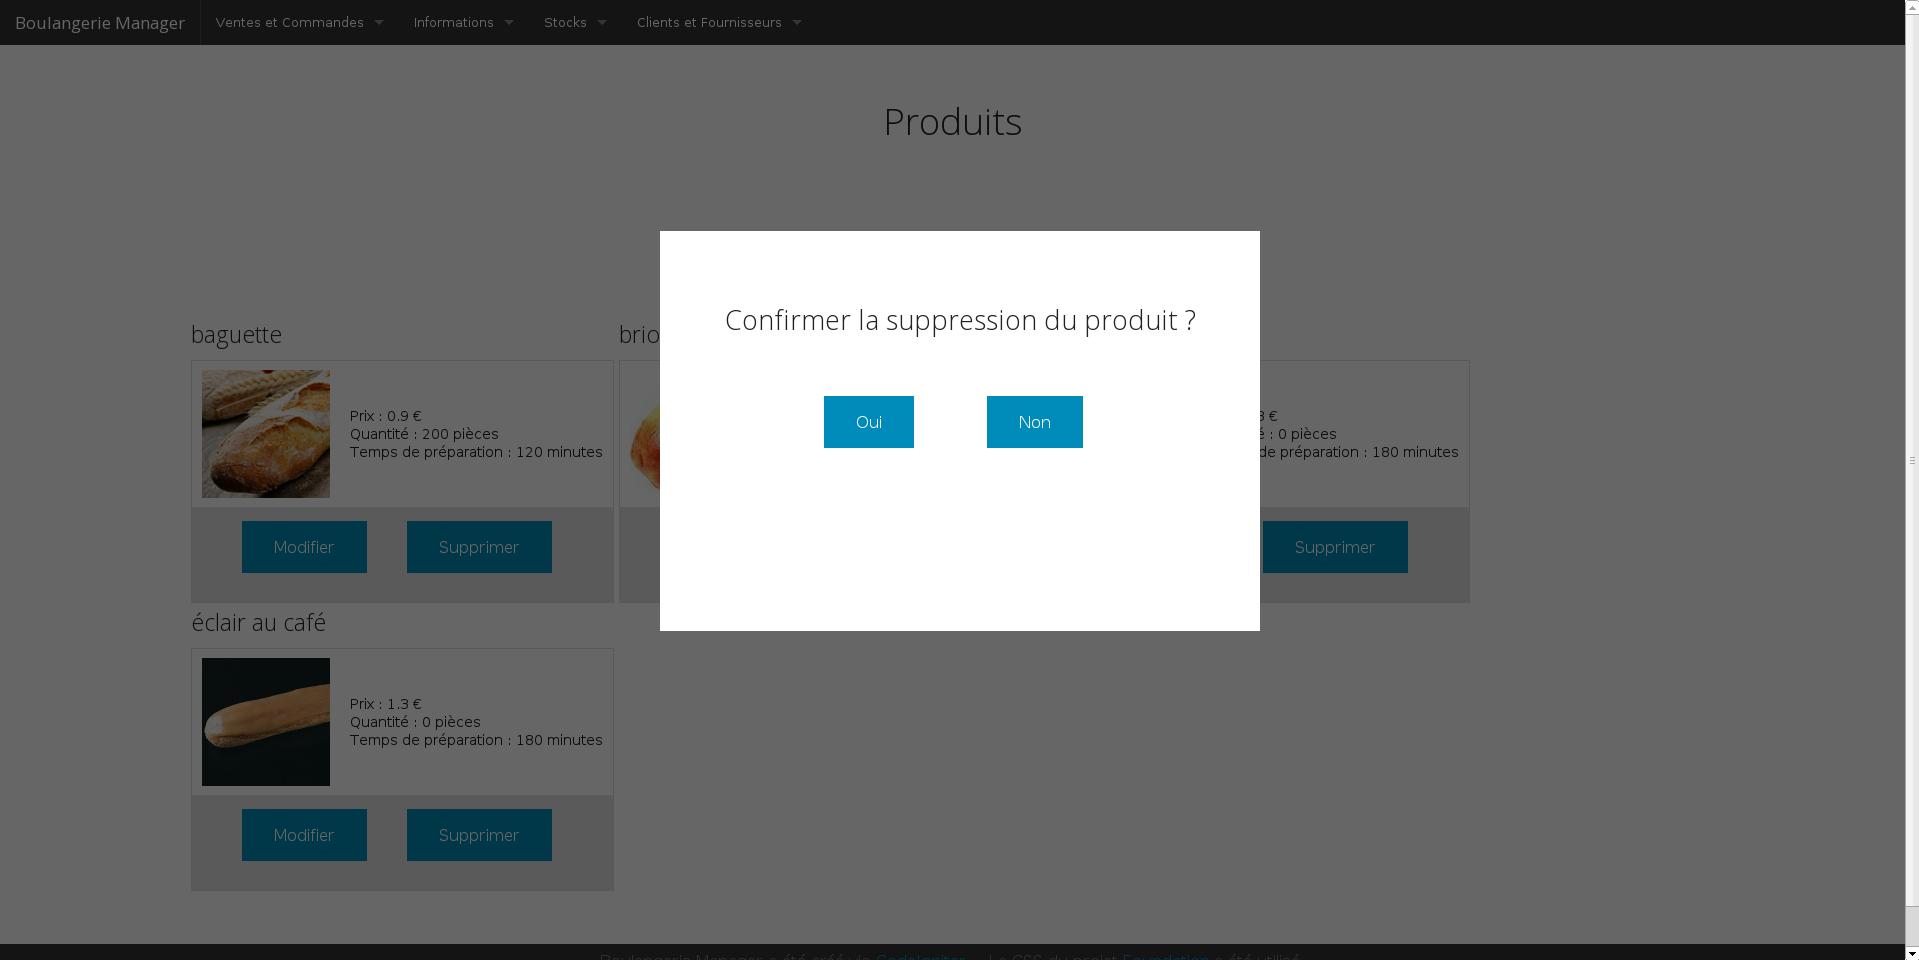
\includegraphics[scale=0.30]{produit3.png}\\
En cliquant sur le bouton "Supprimer" situeé en dessous d'un produit, une 
fenêtre de confirmation apparait nous demande si l'on veut réellement supprimer 
ce produit pour éviter toute erreur possible. Si l'on clique sur "Oui", le 
produit sera supprimé définitivement. Sinon, le produit restera en place et on 
sera renvoyé sur la page principale "Produits".


\subsection{Ajout d'un produit}
Les vignettes associées aux produits sont précédées d'un bouton "Ajouter un 
nouveau produit".

\paragraph{}
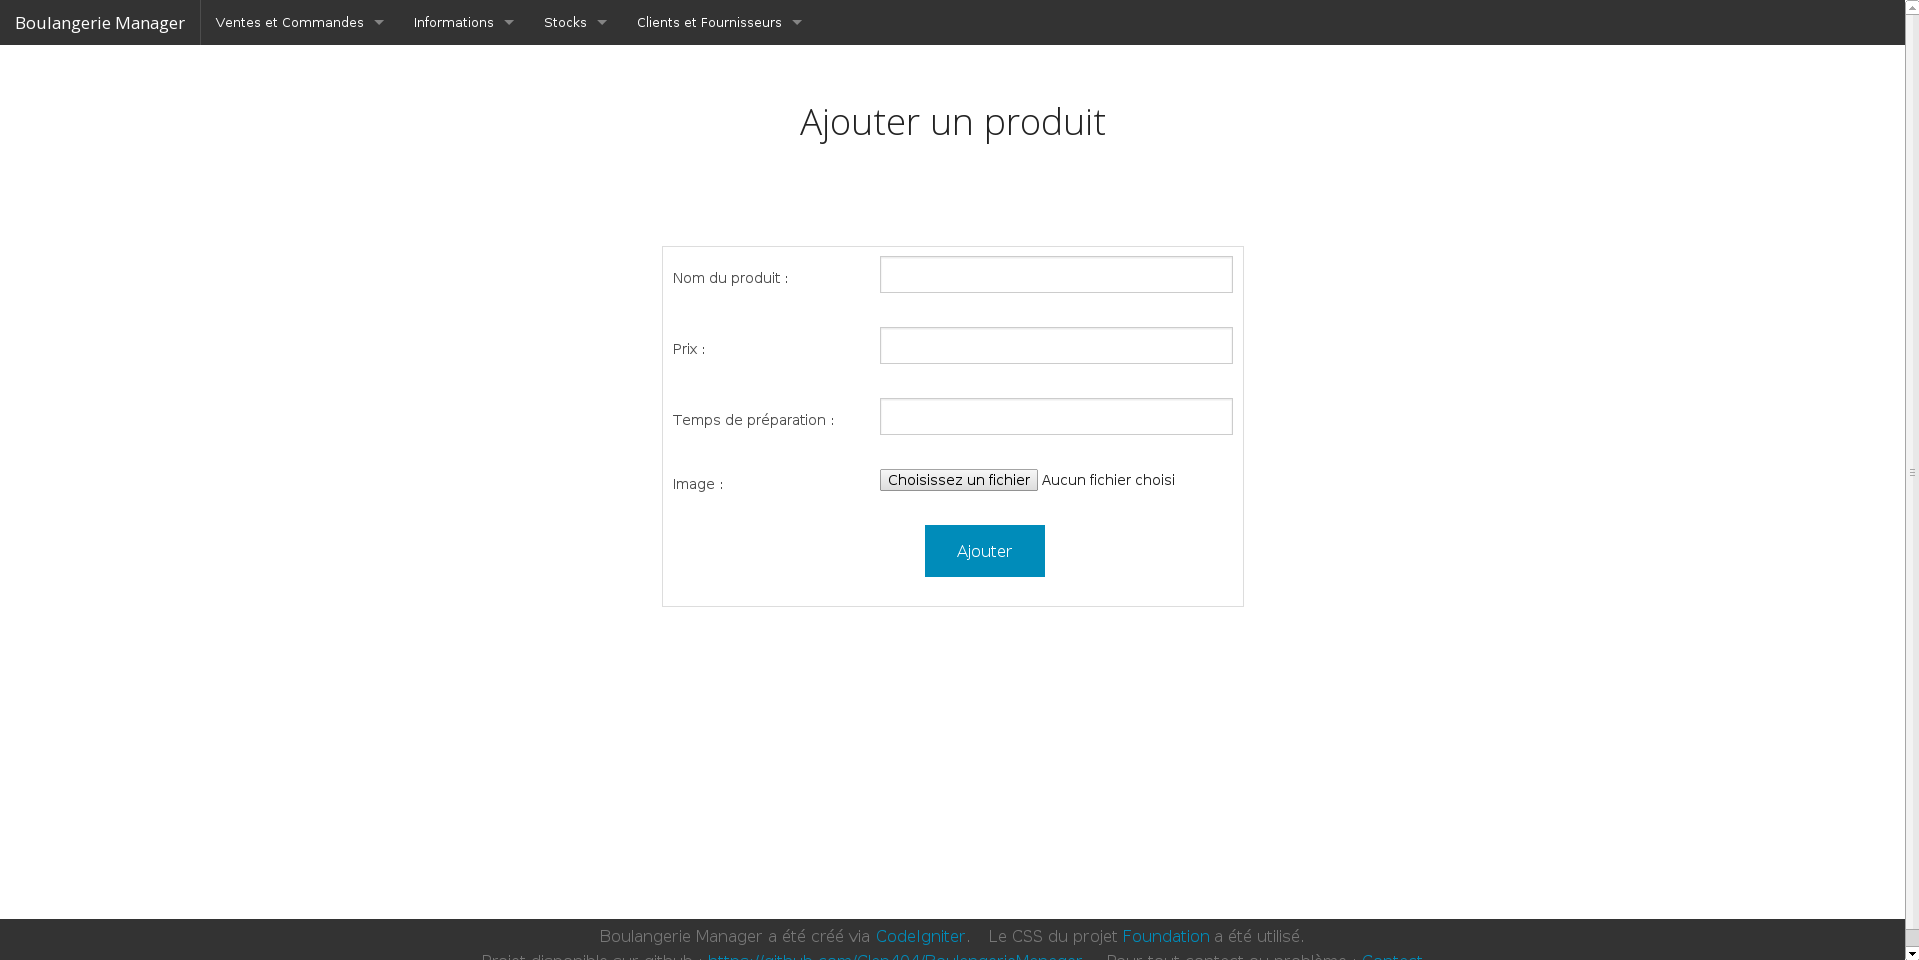
\includegraphics[scale=0.30]{produit4.png}\\
En cliquant sur ce bouton "Ajouter un nouveau produit", une page d'ajout s'ouvre.
Sur cette page d'ajout se trouve trois champs. Le premier champ a renseigner 
représente le nom du produit à ajouter. Le deuxième correspond au prix unitaire 
de ce produit. Le troisième est, quant à lui, le temps de préparation nécéssaire.
Il est également possible d'associer une image à un produit en cliquant sur le 
bouton "Choississez un fichier". En cliquant sur ce bouton, il sera possible de 
charger une image depuis son ordinateur.

\paragraph{}
Si tous les champs ne sont pas remplis, il sera impossible de valider l'ajout de 
produit. S'ils sont bien remplis, un simple clic sur le bouton "Ajouter" 
permet d'ajouter le produit à la liste des produits déjà existants. 



\section{Production}
Cette page permet de renseigner tous les produits qui ont été produits à une date 
donnée.

\subsection{Production d'un produit}
Sur la page "Production" se trouve trois champs à renseigner. Le premier étant 
une date de production. Cette date correspond à la date à laquelle la production 
a eu lieu. Ensuite se trouve le produit qui a été produit. Et le troisième champ 
représente la quantité de produit qui a été produite. Si l'un des trois champs 
n'est pas rempli correctement et que l'on clique sur le bouton "Produire", une 
erreur s'affiche et rien ne se passe. Sinon, la quantité du produit séléctionné 
sera ajouté à la disponibilité de ce produit. Il est également possible de 
produire plusieurs produits de différents types en même temps. En effet, un 
bout "Ajouter une ligne" permet de séléctionner plusieurs produits différents 
et d'en produire des quantités différentes.
